\documentclass{article}
\usepackage[utf8]{inputenc}
\usepackage{hyperref}
\usepackage{url}
\usepackage{graphicx}

\usepackage[backend=bibtex]{biblatex}
\bibliography{ref} 

\title{Smart city ontology: Where are we living?\\ \large Ontologies and Semantic Web: Semester work}
\author{Ondrej Borovec}
\date{October 2018}

\begin{document}

\maketitle

\section{Introduction}

Modern cities are collecting a lot of data to fulfil their majors' promises about SmartCities. Unfortunately most of that data is still stored separately without any level of integration so it does not really server its original purpose. This work if focused on data and ontology about neighbourhood where you live and working with many interesting sources of multiple information fields. Prague - Czech capital - was selected as the best choice to start with, because there are many information sources, which can be used and mined.

Ultimate goal of this work is to design an ontology which covers interesting information about a certen location in a city as weather, parking spot status, future projects or public transportation and traffic limitation. Such information collection can server to anybody, who is looking for a new place for living as well as creating statistics about life quality.

\section{Available data}

Prague has really open policy about sharing data, so there are many sources that can used for the purpose of this semester work. As a research for this, following data access points were used:

\begin{enumerate}
    \item Prague OpenData portal - \cite{opendataprague:online}
    \item Prague Geo portal - \cite{geoportal:online}
    \item Technicka Sprava Komunikaci - \cite{tskpraha:online}
    \item Culture portal Kudy z nudy - \cite{kudyznudy:online}
    \item Culture Prague portal Informuj - \cite{informujpraha:online}
    \item Dopravni podnik mesta Prahy - \cite{dppczRSS:online}
    \item Cesky statisticky urad - \cite{csu:online}
    \item Tenderarena - \cite{tenderarena:online}
\end{enumerate} 

Within this data sources multiple interesting data sets were identified which are listed below in related categories. You can also find exmpales of the data in appendix and the data sets which are seriously considered for further work are recognisable with bold name.

\begin{itemize}
    \item Parking
    \begin{itemize}
        \item \textbf{Parking for handicap people} - \cite{Vyhrazen70:online,Vyhrazen35:online}
        \item Parking for people with special privileges as diplomats or police -  \cite{Vyhrazen81:online}
        \item Parking for suppliers - \cite{Vyhrazen63:online} 
        \item Parking restrictions - \cite{zakazy:online}
        \item \textbf{P+R parking} - \cite{wwwtskpr83:online,Zachytna0:online}
        \item Paid parking - \cite{usekypar48:online,Zonyplac33:online}
    \end{itemize}
    \item Nature
        \begin{itemize}
            \item \textbf{Public parks} - \cite{parky:online}
            \item \textbf{Flooding potential} - \cite{zaplavy:online}
            \item \textbf{Noise} - \cite{hluk1:online,hluk2:online}
        \end{itemize}
    \item Culture - \cite{kudyznudy:online,informujpraha:online}
    \item Ecology
        \begin{itemize}
            \item \textbf{Waste collection} - \cite{Velkoobj59:online,Harmonog59:online,McPraha279:online,Velkoobj47:online}
            \item Separable waste - \cite{Stanovis12:online,Stanovis75:online}
        \end{itemize}
    \item Public transportation
        \begin{itemize}
            \item \textbf{Stops} - \cite{Vstupydo88:online}
            \item Delayes and chanegs - \cite{DPPczZme13:online,DPPczMim53:online}
        \end{itemize}
    \item Economy
        \begin{itemize}
            \item \textbf{Common product price} - \cite{Katalogp90:online}
            \item Flat price - \cite{Sreality94:online,}
        \end{itemize}
    \item Future projects -\cite{tenderarena:online}
    \item Weather - \cite{PortH90:online,Meteosta14:online}
\end{itemize}

Most of the sources can be merged on geo information, but more challenging is the section of Ecology to integrate all tables of all Prague parts and this will be the main focus of this work.


\printbibliography

\appendix

\section{Ecology data examples}
\begin{figure}[h]
    \centering
    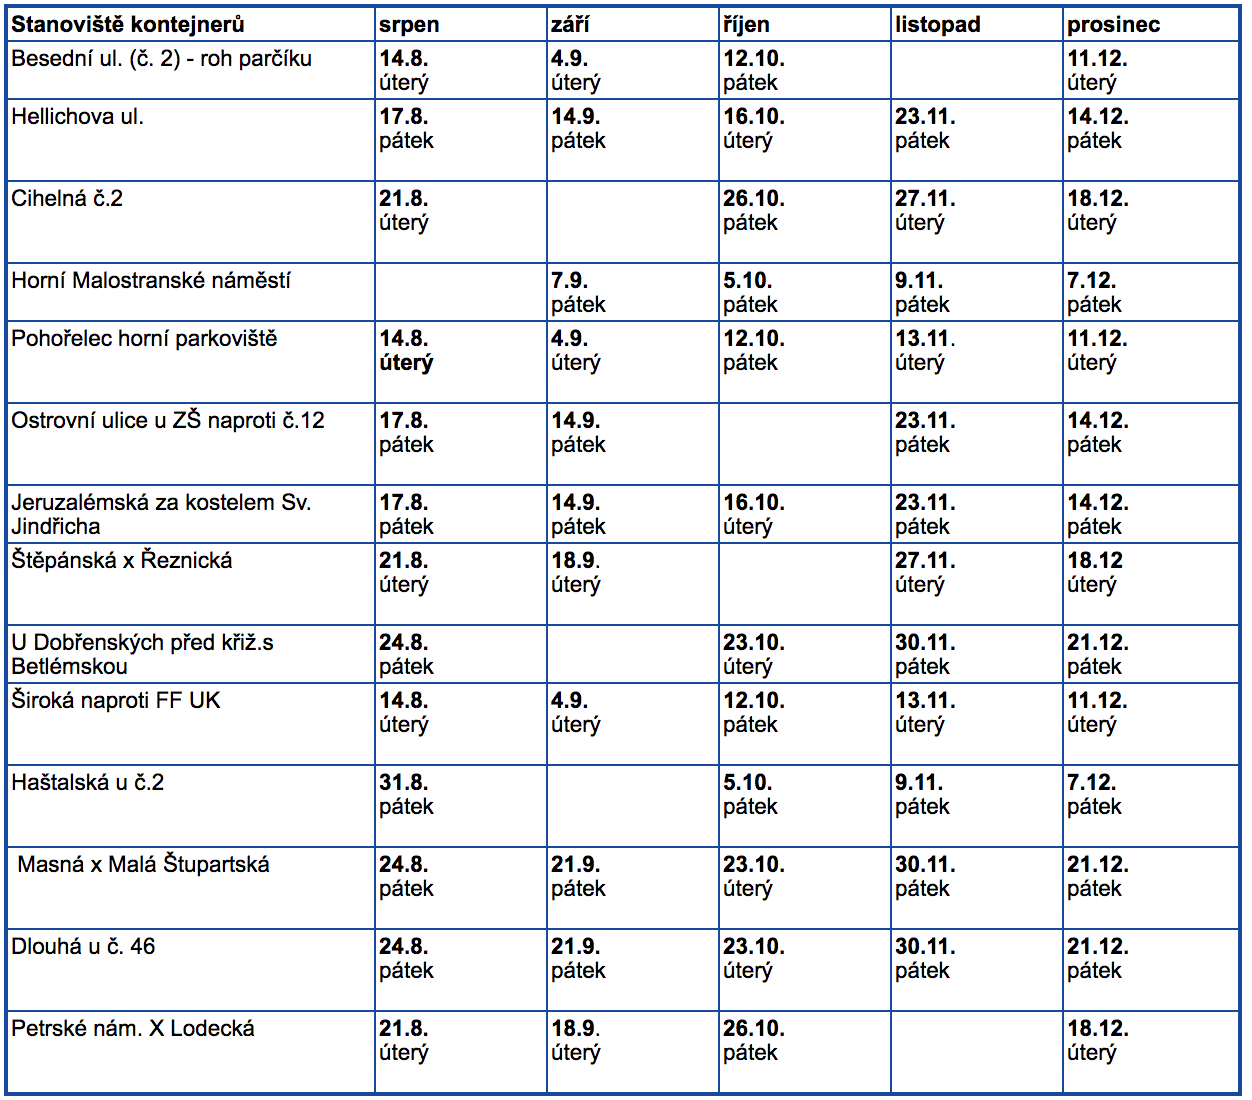
\includegraphics[width=0.8\textwidth]{imgs/praha1.png}
    \caption{Screen-shot of schedule from \cite{Harmonog59:online}}
\end{figure}
\begin{figure}[h]
    \centering
    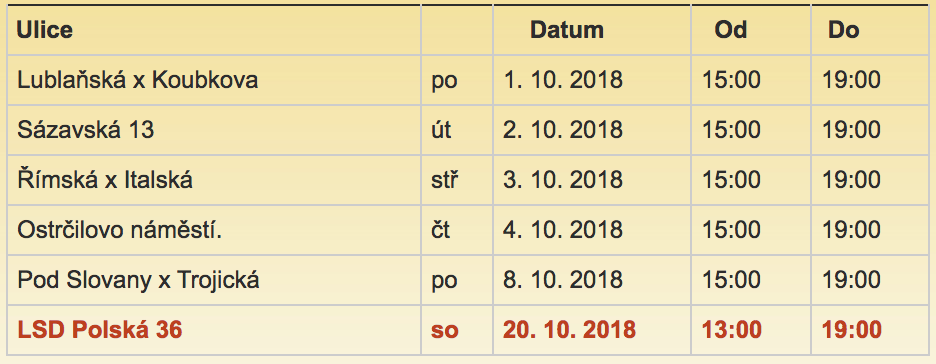
\includegraphics[width=0.8\textwidth]{imgs/praha2.png}
    \caption{Screen-shot of schedule from \cite{McPraha279:online}}
\end{figure}
\end{document}
